\subsection{Preparation of the Input}

In this section we focus on predicting both real and imaginary parts of the \texttt{exp} label using both the lumps and the \wzw datasets together: the idea is to have a model independent architecture able to make predictions without knowledge of the underlying physical model.
In fact we will also use part of the double lump solutions to make sure that the \ml models are properly independent on the physical models underlying the data.

The datasets of the lumps and \wzw models are however defined differently and many variables differ in the two physical models.
We start from the tidy datasets which have been prepared for the separate analysis in the previous sections.

We will proceed as follows, before merging the datasets:
\begin{itemize}
  \item we transform the columns in the lumps dataset to account for the imaginary parts of the truncation levels (identically vanishing), that is we add columns corresponding to the imaginary part of the truncation levels,
  \item we compute the PCA of the truncation levels in both datasets, keeping 10 components each to maximise the retained variance,
  \item we then select the \texttt{weight}, \texttt{type} and the PCA variables in both datasets,
  \item we \emph{outer join} the datasets on the \texttt{weight} and \texttt{type} variables.
\end{itemize}
We finally have a new dataset containing 12 features and 2 labels (i.e.\ $\Re(exp)$ and $\Im(exp)$), and 2379 samples.

We then prepare the dataset containing data on the double lump solutions.
First of all we select only data with weight $h < 1.5$ for reliability.
We then apply the same transformations described earlier, but we do not immediately merge the data with the previous dataset.
Since these data come from a different model but refer to only one solution, we keep them separate and use them mainly for evaluation purposes in the validation and test sets used in the analysis.

The final result of the preparation is as follows:
\begin{itemize}
  \item one dataset containing 12 features and 2 labels across 2379 samples (i.e.\ lumps and \wzw data),
  \item one dataset containing 12 features and 2 labels with 12 samples (i.e.\ the double lumps).
\end{itemize}
We can now move to the analysis of the machine learning algorithms.
We first need to define a validation strategy for the different datasets.


\subsection{Validation Strategy}

For the analysis we keep in general \SI{80}{\percent} of the samples for training, \SI{10}{\percent} for validation and \SI{10}{\percent} as a test set as we did before for the two separate datasets.
In this case the datasets can be freely shuffled since all the information on the model is already encoded in the variables.\footnotemark{}
\footnotetext{%
  That is we do not need to add a \texttt{solutions} column and use that to separate the samples.
}

However we treat the double lumps dataset in a different way.
The steps necessary to reproduce the input datasets are as follows:
\begin{itemize}
  \item take the joined dataset with lumps and \wzw data and sample it with \SI{80}{\percent} of the data for the training set, \SI{10}{\percent} for the validation set, \SI{10}{\percent} for the test set,
  
  \item take the double lumps data and split it in half: insert the first half in the validation set, and the second half in the test set.
\end{itemize}

Before passing the input to the algorithms we scale it using the \texttt{StandardScaler} class in \texttt{Scikit-learn} in order to standardise the features and simplify the learning process.
We also scale the labels to contain the range of variability of the predictions.\footnotemark{}
\footnotetext{%
  Predictions will not be directly comparable, but we must remember to scale any new data before computing the metrics.
}
For this we use the \texttt{MinMaxScaler} class in \texttt{Scikit-learn}.
In both cases we fit the transformers on the training set and then apply the transformation to the validation and test sets.\footnotemark{}
\footnotetext{%
  We do not simply divide the data by a constant arbitrary number because that would not change anything in the algorithms.
  It would also add a bias in the analysis, since there is no way to predict what constant factor to use.
}

We focus on predicting both $\Re(exp)$ and $\Im(exp)$ at the same time with a single model.
We will use and compare \emph{r-SVM}s, \emph{GBDT}s and \emph{ANN}s models.
However, since the first two algorithms cannot naturally account for two outputs, we use the \texttt{MultiOutputRegressor} class in \texttt{Scikit-learn} which automatically uses the same estimator to predict separately both labels.

We adopt two different validations strategies.
In fact, for support vector machines and gradient boosted trees we use a cross validation strategy: we join the training and validation sets in this case to have \SI{90}{\percent} of data in total for training and validation.
We adopt \num{9}-folds cross validation to always have \SI{10}{\percent} of the data for evaluation.
Thus we will in general train the algorithm on \num{8} folds and evaluate on the \num{9}th: every time there will be a chance to train on the double lumps data which might help the algorithms to predict also those solutions.


\subsection{Support Vector Machines}

\subsubsection{Training}

The model used for training is a single architecture to predict both real and imaginary parts of \texttt{exp}.
Since we use a cross validation strategy, we perform the automatic optimisation of the hyperparameters using the \texttt{BayesSearchCV} class in \texttt{Scikit-optimize}, which uses Bayes optimisation to look for the best hyperparameters.
In the end the best hyperparameters chosen to predict both real and imaginary parts of \texttt{exp} are $C = 12$, $\epsilon = 0$, and $\gamma = 10$.\footnotemark{}
\footnotetext{%
  $C$ refers to the penalty assigned to samples outlying the \emph{no penalty} margin of support vectors, $\epsilon$ to the soft margin width, and $\gamma$ to the width of the Gaussian kernel.
}


\subsubsection{Results}

Results on the test fold are summarised in \Cref{tab:agg:svr_met}.
In general the algorithm performs better on the imaginary part of the label, but results are good also for the real part.

\begin{table}[htbp]
  \centering
  %\resizebox{\textwidth}{!}{%
  \begin{tabular}{@{}cccc@{}}
  \toprule
             & \mse    & \mae  & \rr   \\
  \midrule
  $\Re(exp)$ & 0.01    & 0.04  & 0.84  \\
  $\Im(exp)$ & 0.0005  & 0.004 & 0.97  \\
  \bottomrule
  \end{tabular}%
  %}
  \caption{Summary of the metrics of the \emph{r-SVR} on the test set.}
  \label{tab:agg:svr_met}
\end{table}

In \Cref{fig:agg:svr_pred} we show the predictions of the real and imaginary parts of \texttt{exp} using the \emph{r-SVR} algorithm.
As we can see most of the predictions are correctly reproduced by the weights of the support vectors.
Some predictions are slightly underestimated in the real part of the label, but the residual plot in \Cref{fig:agg:svr_res_plot} shows that the residuals are however contained.

\begin{figure}[htbp]
  \centering
  \begin{subfigure}{0.45\textwidth}
    \centering
    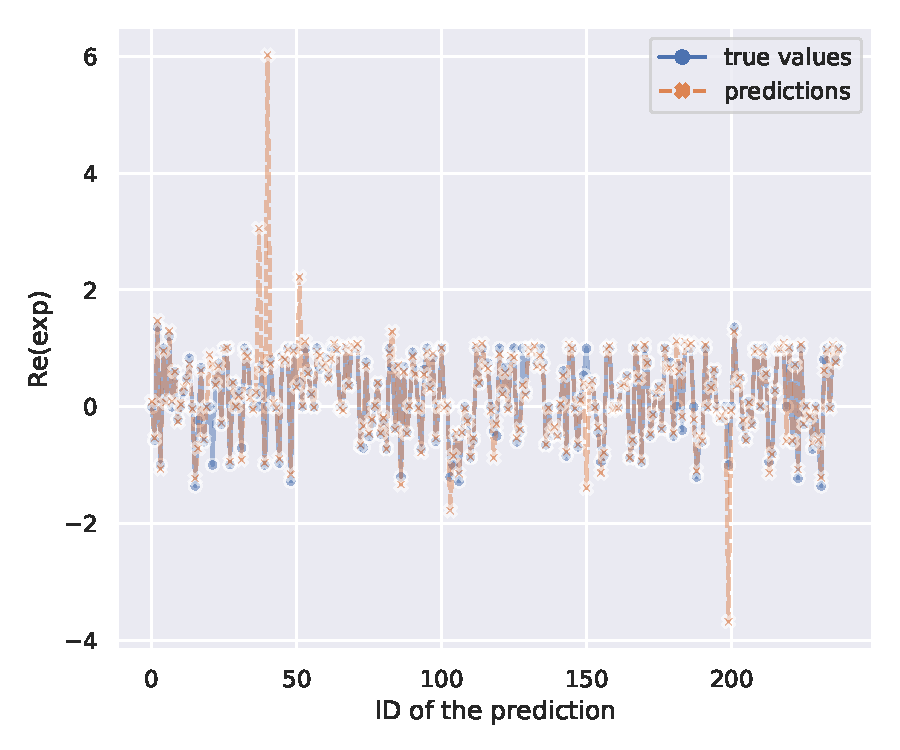
\includegraphics[width=\linewidth]{img/svr_test_exp_re_plot}
    \caption{Real part.}
  \end{subfigure}
  \begin{subfigure}{0.45\textwidth}
    \centering
    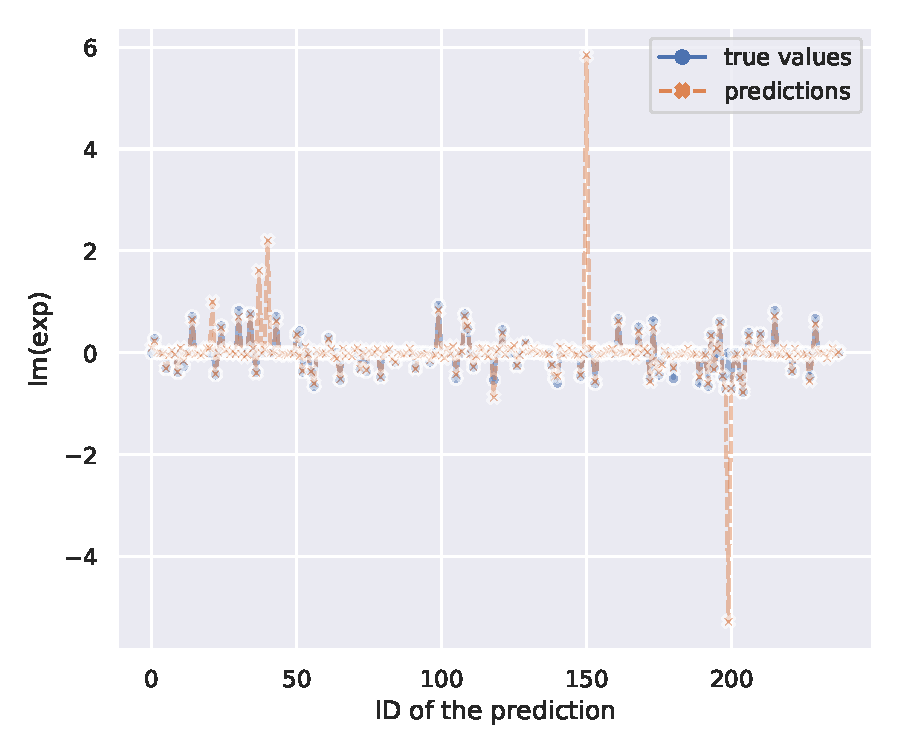
\includegraphics[width=\linewidth]{img/svr_test_exp_im_plot}
    \caption{Imaginary part.}
  \end{subfigure}
  \caption{Predictions and true values using the \emph{r-SVR} algorithm.}
  \label{fig:agg:svr_pred}
\end{figure}

\begin{figure}[htbp]
  \centering
  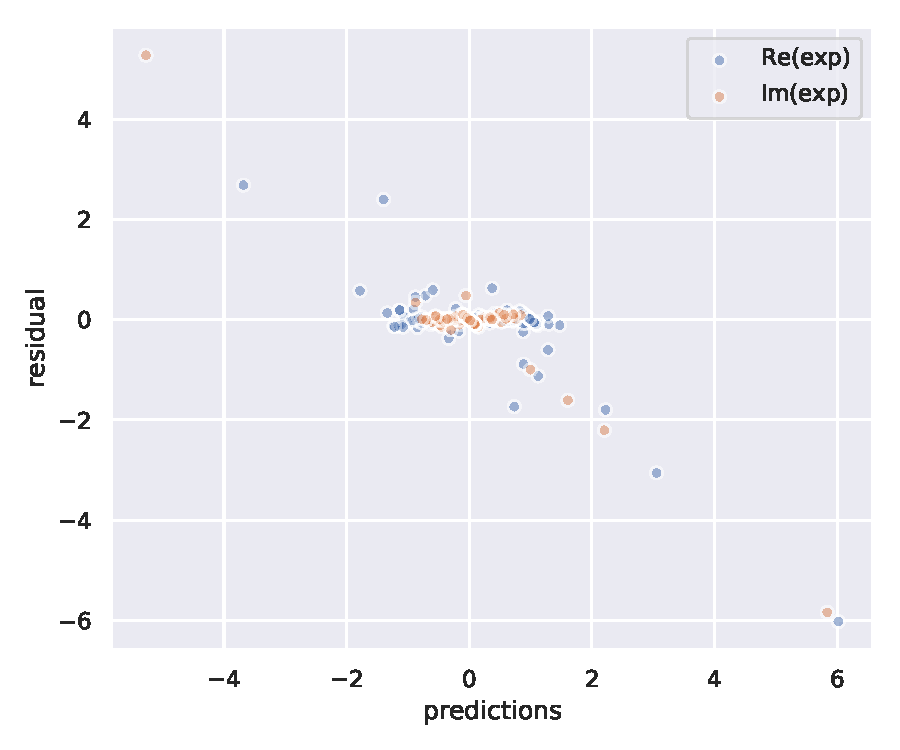
\includegraphics[width=0.6\textwidth]{img/svr_test_res_plot}
  \caption{Residual plot using the \emph{r-SVR}.}
  \label{fig:agg:svr_res_plot}
\end{figure}


\subsection{Gradient Boosted Decision Trees}

\subsubsection{Training}

We use the same training strategy of the \emph{r-SVR} algorithm.
The optimal hyperparameters are: \texttt{colsample\_bytree} $= 0.7$, \texttt{learning\_rate} $= 0.01$, \texttt{max\_depth} $= 25$, \texttt{min\_child\_weight} $= 0.1$, \texttt{n\_estimators} $= \num{50000}$, \texttt{num\_leaves} $= 25$, \texttt{reg\_alpha} $= 1.0$, \texttt{reg\_lambda} $= \num{1000}$, \texttt{subsample} $= 0.99$.\footnotemark{}
\footnotetext{%
  \texttt{colsample\_bytree} refers to the fraction of features used in each tree, the \texttt{learning\_rate} to the shrinking parameters used in the gradient descent, \texttt{max\_depth} is the maximal amount of branches in each tree, \texttt{min\_child\_weight} is the minimum number of samples to branch the tree, \texttt{n\_estimators} is the number of boosting round, \texttt{num\_leaves} is the number of leaves in each branch, \texttt{reg\_alpha} is the amount of $\ell_1$ regularisation, \texttt{reg\_lambda} is the amount of $\ell_2$ regularisation, and \texttt{subsample} is the fraction of samples used.
}


\subsubsection{Results}

Results on the test sets are shown in \Cref{tab:agg:gbdt_met}.

\begin{table}[htbp]
  \centering
  %\resizebox{\textwidth}{!}{%
  \begin{tabular}{@{}cccc@{}}
  \toprule
             & \mse    & \mae  & \rr   \\
  \midrule
  $\Re(exp)$ & 0.007   & 0.03  & 0.89  \\
  $\Im(exp)$ & 0.0014  & 0.012 & 0.93  \\
  \bottomrule
  \end{tabular}%
  %}
  \caption{Summary of the metrics of the \emph{GBDT} on the test set.}
  \label{tab:agg:gbdt_met}
\end{table}

In \Cref{fig:agg:gbdt_pred} we show the predictions of the real and imaginary parts of \texttt{exp}.
As in the previous case, some predictions are slightly underestimated in the real part of the label, but the residual plot in \Cref{fig:agg:gbdt_res_plot} shows that the residuals are however contained.

\begin{figure}[htbp]
  \centering
  \begin{subfigure}{0.45\textwidth}
    \centering
    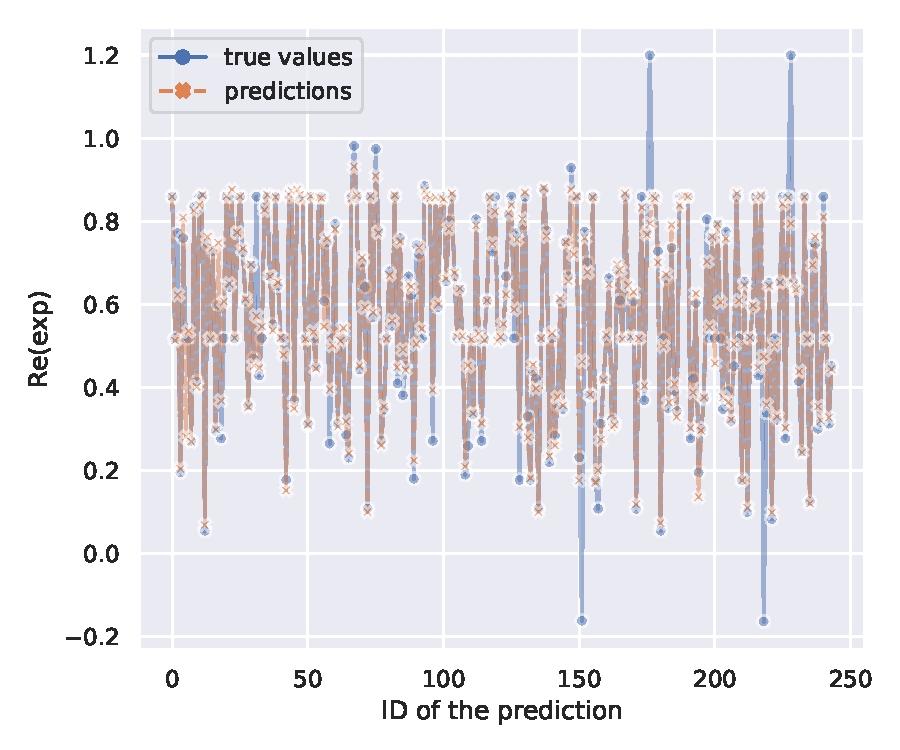
\includegraphics[width=\linewidth]{img/gbdt_test_exp_re_plot}
    \caption{Real part.}
  \end{subfigure}
  \begin{subfigure}{0.45\textwidth}
    \centering
    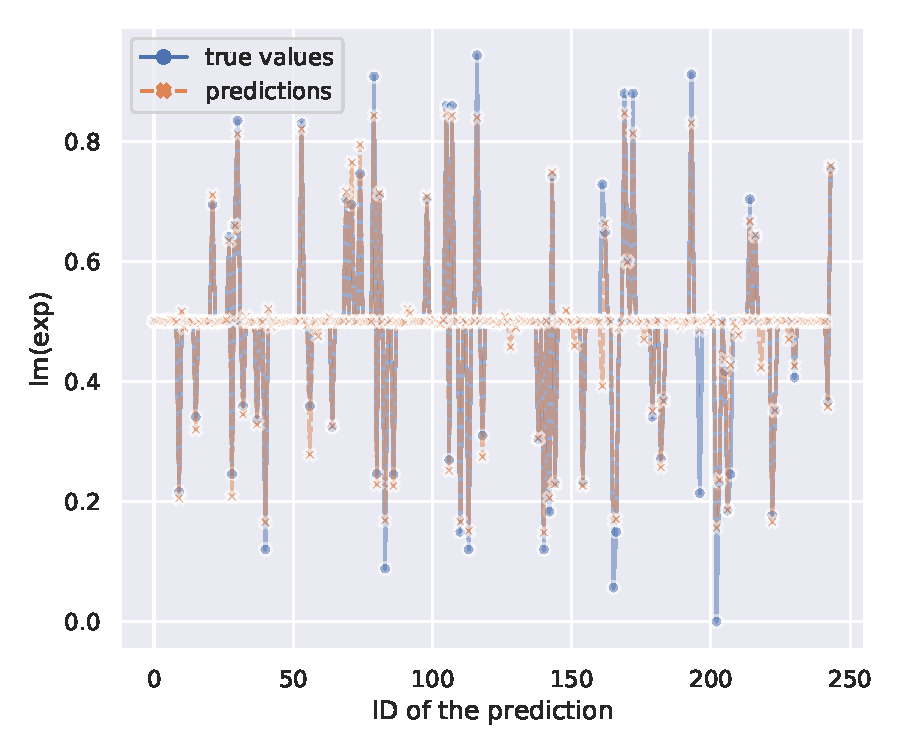
\includegraphics[width=\linewidth]{img/gbdt_test_exp_im_plot}
    \caption{Imaginary part.}
  \end{subfigure}
  \caption{Predictions and true values using the \emph{GBDT} algorithm.}
  \label{fig:agg:gbdt_pred}
\end{figure}

In general we can see that the real part of the label is better approximated by the \emph{GBDT}, which however suffers a bit more in the imaginary part with respect to the \emph{r-SVR}.
In general the results are very good since the coefficient of determination \rr is well above \num{0.8} for both the labels.

\begin{figure}[htbp]
  \centering
  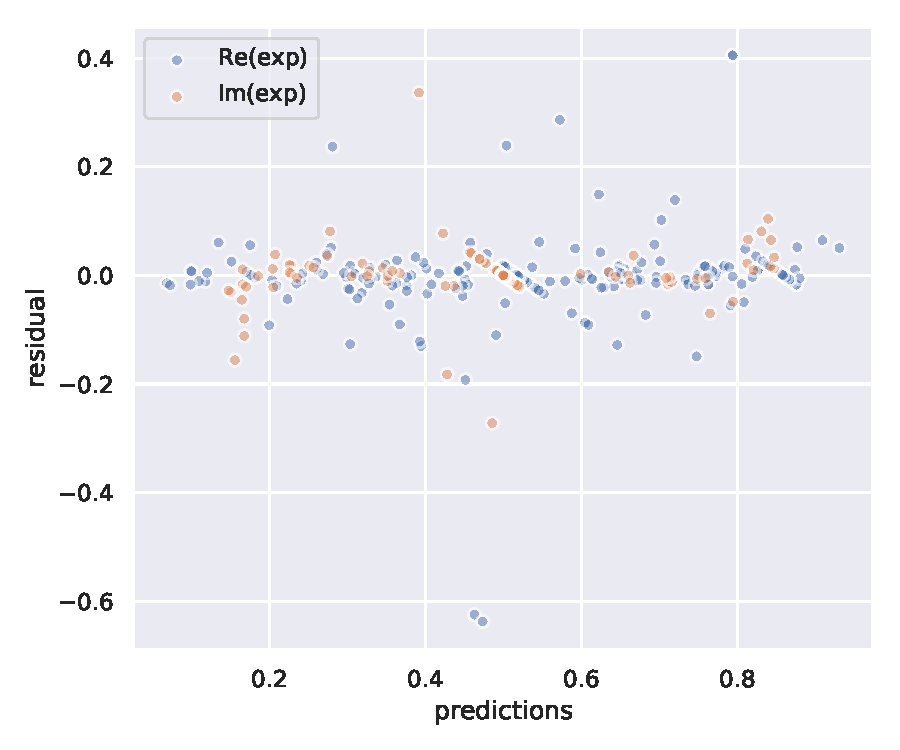
\includegraphics[width=0.6\textwidth]{img/gbdt_test_res_plot}
  \caption{Residual plot using the \emph{GBDT}.}
  \label{fig:agg:gbdt_res_plot}
\end{figure}


\subsection{Artificial Neural Network}

\subsubsection{Model}

The model we use for training is a simple fully connected network (summarised in \Cref{tab:agg:keras_summary}).
The architecture is made of 4 hidden layers with \numlist{50;50;10;10} units each and dropout layers (with rate \num{0.05}) after the first two hidden layers (see \Cref{fig:agg:arch}).
Each hidden fully connected layer is followed by a ReLU activation function.
The addition of batch normalisation layers drastically increased the error, so we dropped them entirely in this implementation.
The output layers are two separate fully connected layers with 1 unit each containing $\Re(exp)$ and $\Im(exp)$.
No regularisation was introduced.

\begin{table}[htbp]
  \centering
  \begin{tabular}{@{}lcc@{}}
    \toprule
    \textbf{layer}               & \textbf{shape} & \textbf{parameters} \\
    \midrule
    \emph{input}                 & (12,)          & 0                   \\
    \emph{fully connected}       & (50,)          & 390                 \\
    \emph{dropout}               & (50,)          & 0                   \\
    \emph{fully connected}       & (50,)          & 930                 \\
    \emph{dropout}               & (50,)          & 0                   \\
    \emph{fully connected}       & (10,)          & 310                 \\
    \emph{fully connected}       & (10,)          & 110                 \\
    $\Re(exp)$ (\emph{output})   & (1,)           & 11                  \\
    $\Im(exp)$ (\emph{output})   & (1,)           & 11                  \\
    \midrule
    \emph{Total parameters:}     & \num{3842}     &                     \\
    \emph{Trainable parameters:} & \num{3842}     &                     \\
    \bottomrule
  \end{tabular}
  \caption{Summary of the network.}
  \label{tab:agg:keras_summary}
\end{table}

\begin{figure}[htbp]
  \centering
  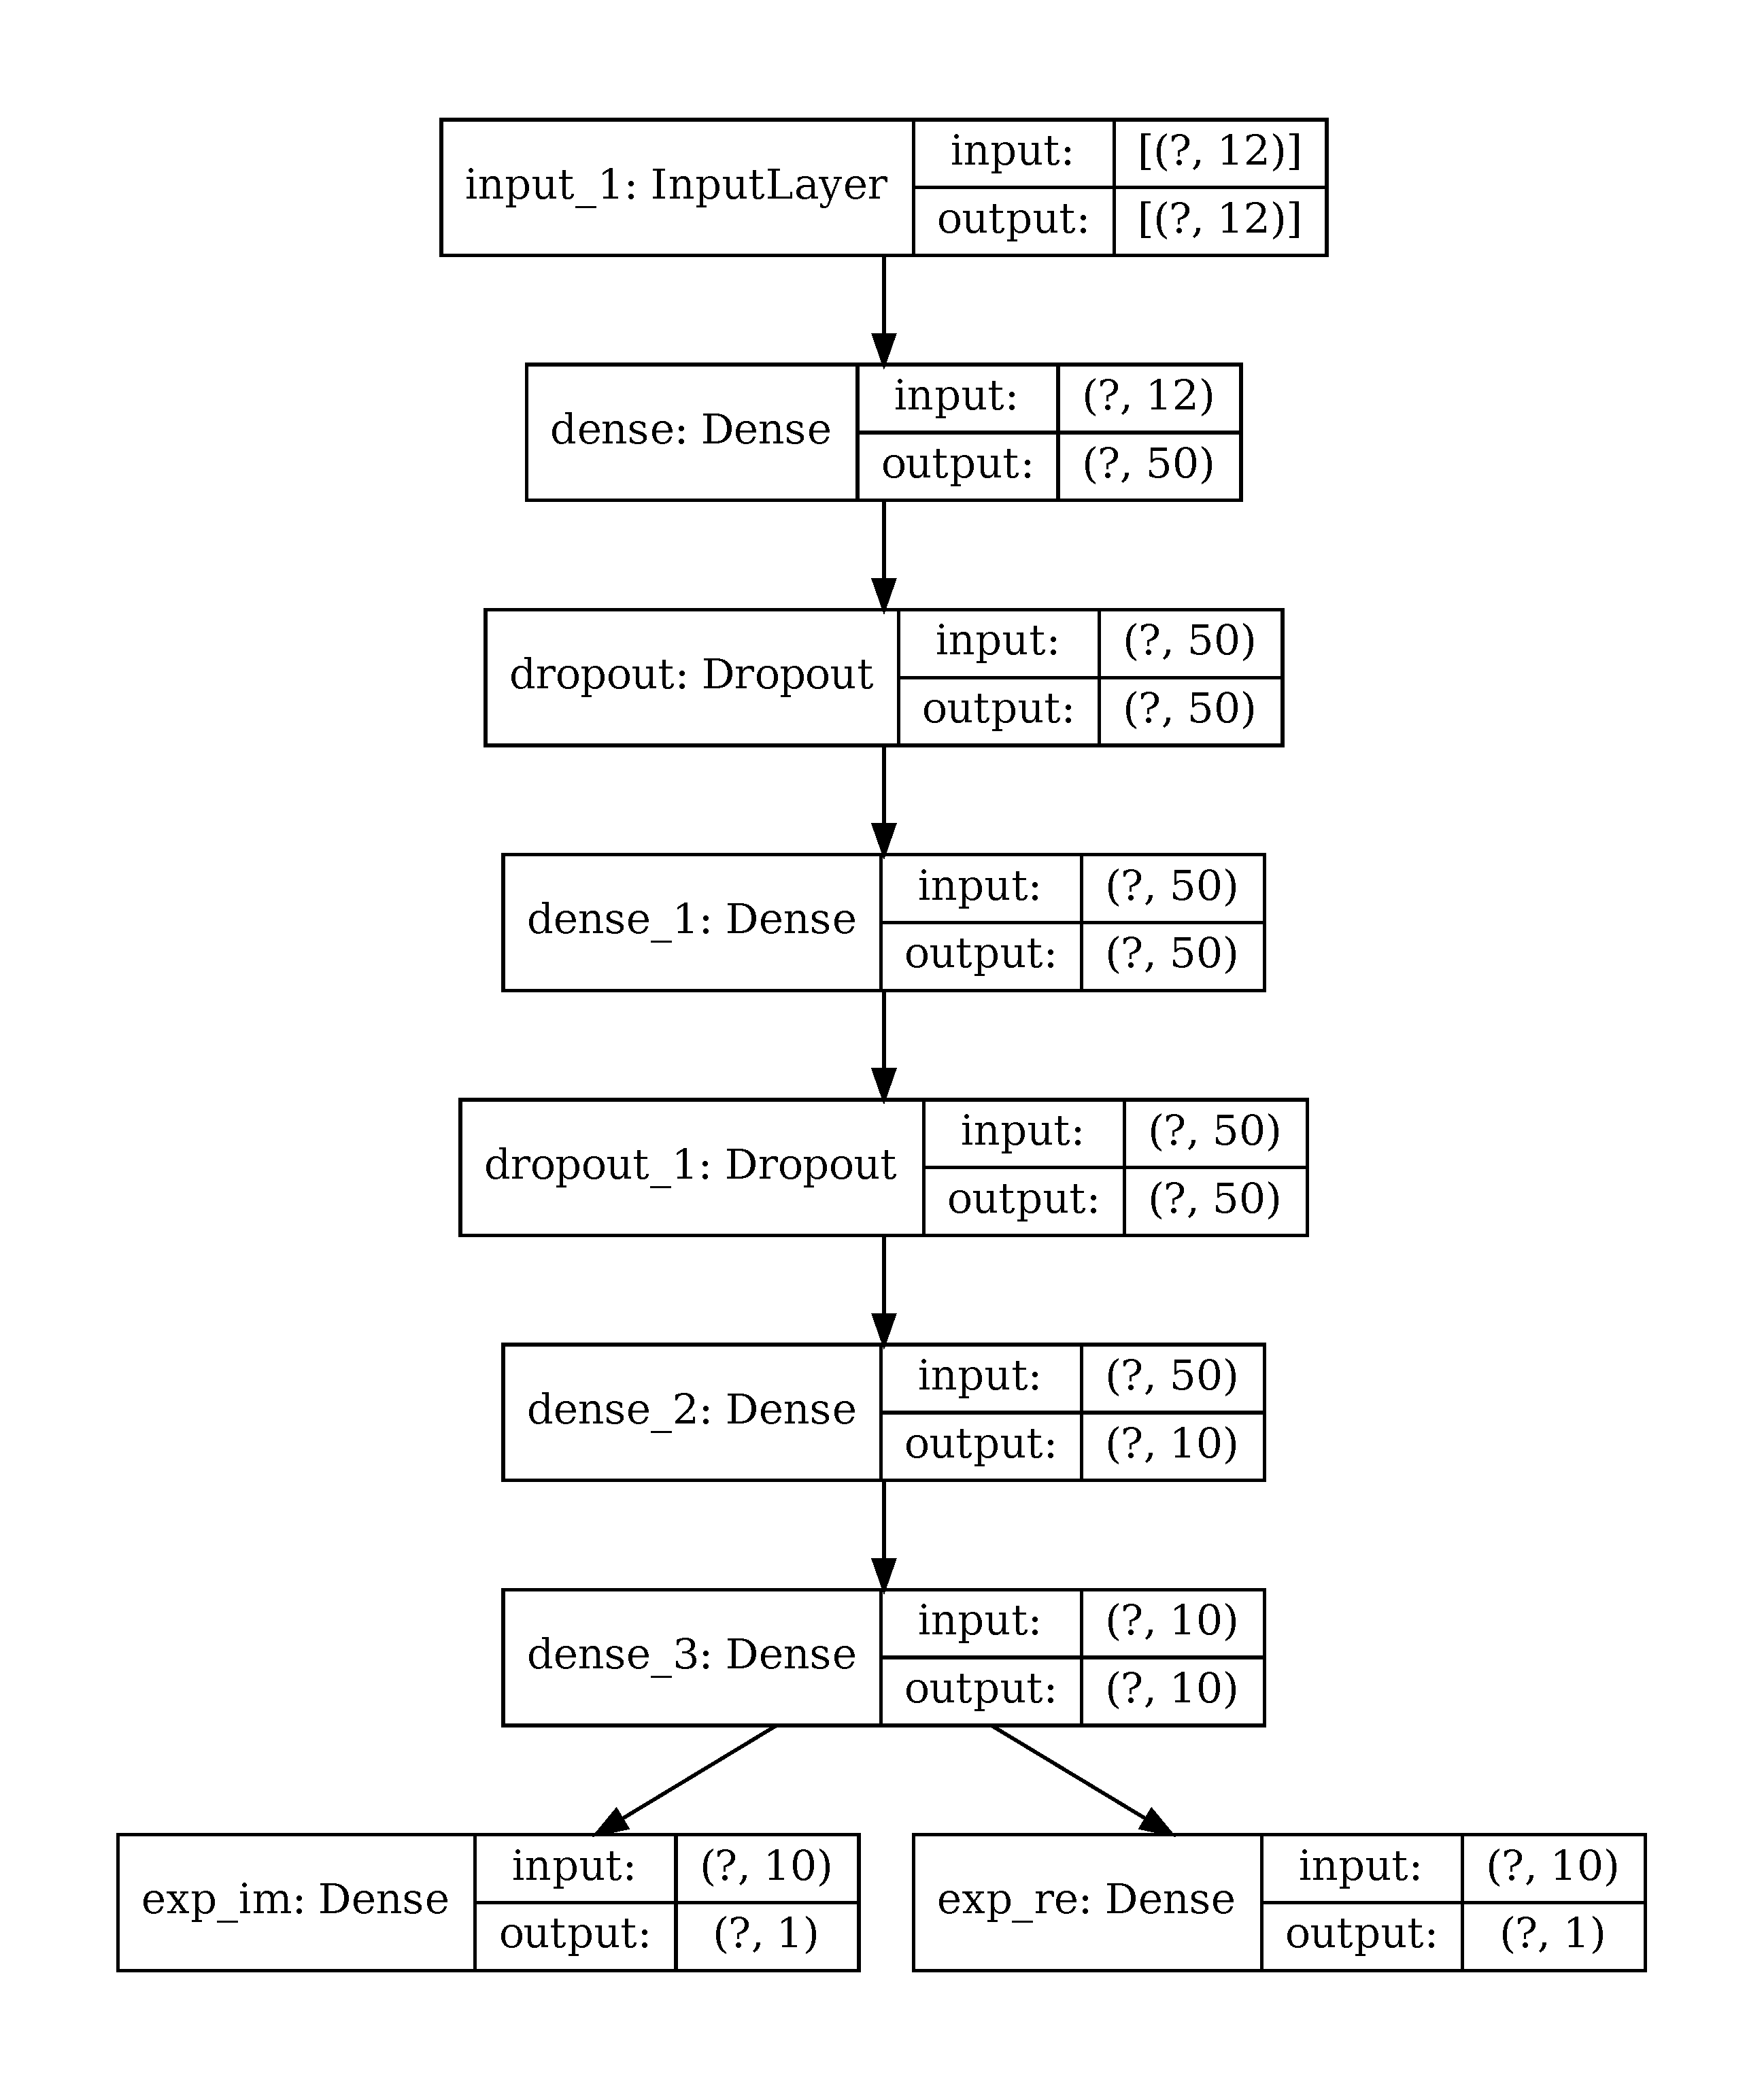
\includegraphics[width=0.6\textwidth]{img/ann_arch}
  \caption{Architecture of the ANN.}
  \label{fig:agg:arch}
\end{figure}


\subsubsection{Training}

For training we use the \mse as loss function and weigh it on the two output layers with \numlist{0.75;0.25} loss weights for the real and imaginary part of the \texttt{exp} label respectively.\footnotemark{}
\footnotetext{%
  The loss function must be a scalar metric, thus the \mse in this case is separately computed on the output layers and then combined by multiplying each loss by the corresponding weight.
  Clearly the sum of all weights should be the unit.
}
For gradient descent we use the \emph{Adam} optimiser with default values and initial learning rate of \num{0.001} and a mini batch size of 32.
The maximal number of epochs used for training is \num{20000} but it greatly exceeds what actually needed for good results.
In fact we also implement a callback to early stop the training after 1000 epochs without improvement of the loss function on the validation data.
We finally add a callback to reduce the learning rate by a step factor of \num{0.3} after 750 epochs without improvement on the validation loss.

The loss function and the \mse are displayed in log scale in \Cref{fig:agg:err}.
They show a drastic drop in error and loss around 100 epochs of training and a stabilisation after that.
Early stopping the network has also the regularisation effect of avoiding the overfit of the traning set.

\begin{figure}[htbp]
  \centering
  \begin{subfigure}{0.45\textwidth}
    \centering
    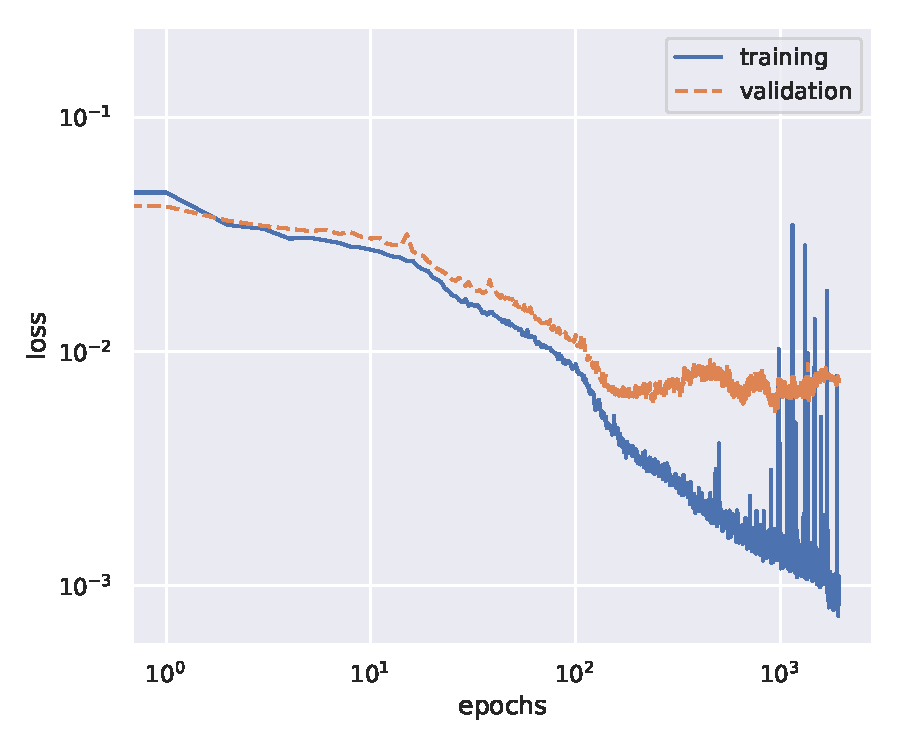
\includegraphics[width=\linewidth]{img/loss}
    \caption{Weighted loss.}
  \end{subfigure}
  \begin{subfigure}{0.45\textwidth}
    \centering
    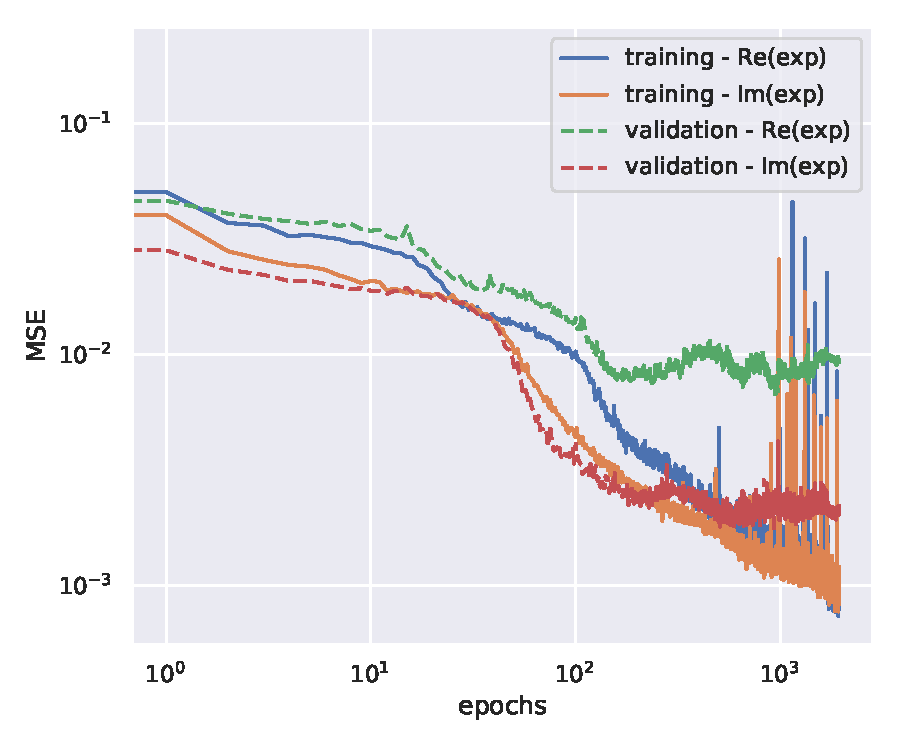
\includegraphics[width=\linewidth]{img/mse}
    \caption{\mse metric.}
  \end{subfigure}
  \caption{Loss function and errors (log scale).}
  \label{fig:agg:err}
\end{figure}

Differently from the cross validation strategy adopted for \emph{r-SVR} and \emph{GBDT}, for the \emph{ANN} we inserted the double lump solutions only in the validation and test sets.
The algorithm is therefore trained only on lumps and \wzw model but evaluated on all real world scenarios.


\subsubsection{Results}

The metrics computed on the test set are shown in \Cref{tab:agg:ann_metrics}.
The results are in general good and the coefficient of determination \rr is very high for both labels.
Comparing with the results in the validation set ($\rr = 0.89$ for $\Re(exp)$ and $\rr = 0.89$ for $\Im(exp)$), it seems that the architecture does not overfit the validation set.\footnotemark{}
\footnotetext{%
  This is in general a risk when using a single validation set.
}

\begin{table}[htbp]
  \centering
  %\resizebox{\textwidth}{!}{%
  \begin{tabular}{@{}cccc@{}}
  \toprule
             & \mse   & \mae  & \rr   \\
  \midrule
  $\Re(exp)$ & 0.010  & 0.03  & 0.84  \\
  $\Im(exp)$ & 0.0008 & 0.016 & 0.95  \\
  \bottomrule
  \end{tabular}%
  %}
  \caption{Metrics of the \emph{ANN} computed on the test set.}
  \label{tab:agg:ann_metrics}
\end{table}

In fact, \Cref{fig:agg:ann_preds} shows that the agreement between predictions and true values in the test set is very good.
It also does not show signs of isolated samples producing a completely wrong predictions as for the \emph{r-SVR}.
Taking a look at the residuals we can also see that the errors are in general well distributed and do not show sign of patterns (see \Cref{fig:agg:ann_res}).

\begin{figure}[htbp]
  \centering
  \begin{subfigure}{0.45\textwidth}
    \centering
    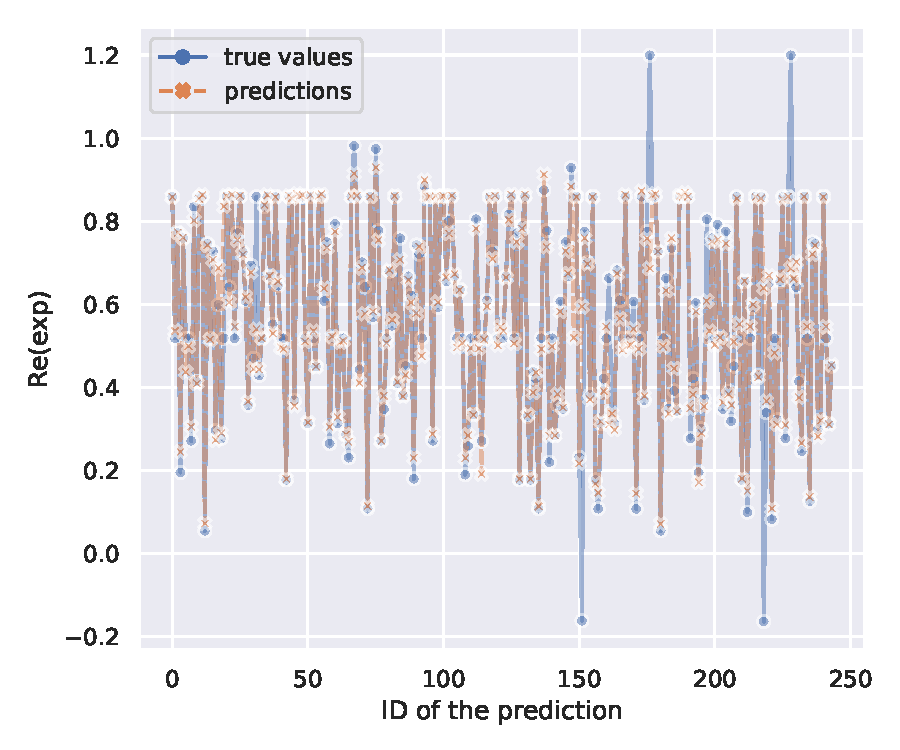
\includegraphics[width=\linewidth]{img/test_exp_re_plot}
    \caption{Real part.}
  \end{subfigure}
  \begin{subfigure}{0.45\textwidth}
    \centering
    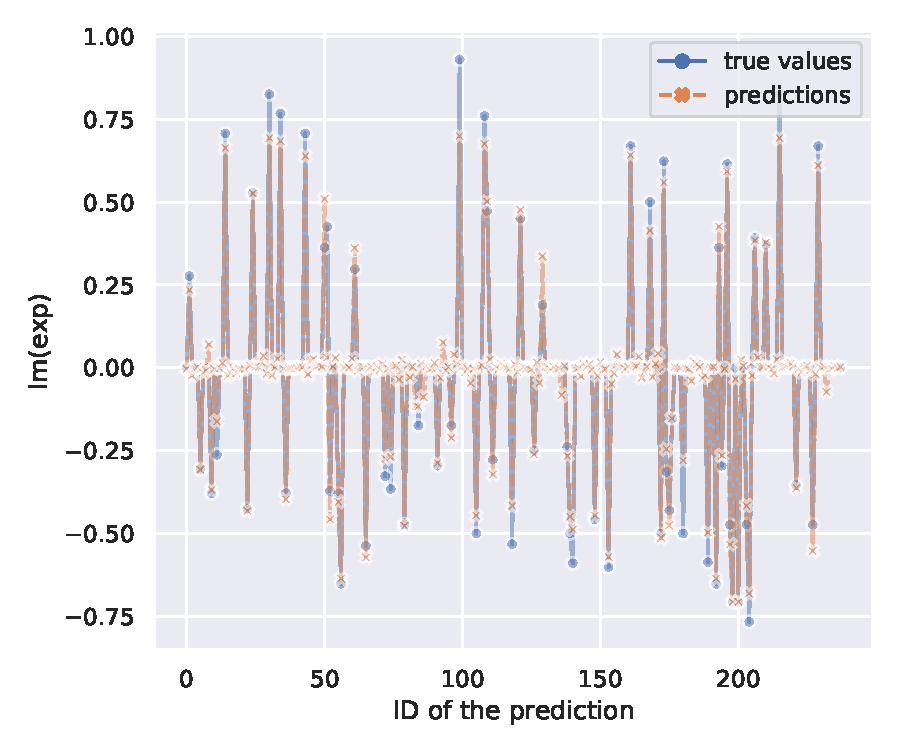
\includegraphics[width=\linewidth]{img/test_exp_im_plot}
    \caption{Imaginary part.}
  \end{subfigure}
  \caption{Predictions and true values using the \emph{ANN} model.}
  \label{fig:agg:ann_preds}
\end{figure}

\begin{figure}[htbp]
  \centering
  \begin{subfigure}{0.45\textwidth}
    \centering
    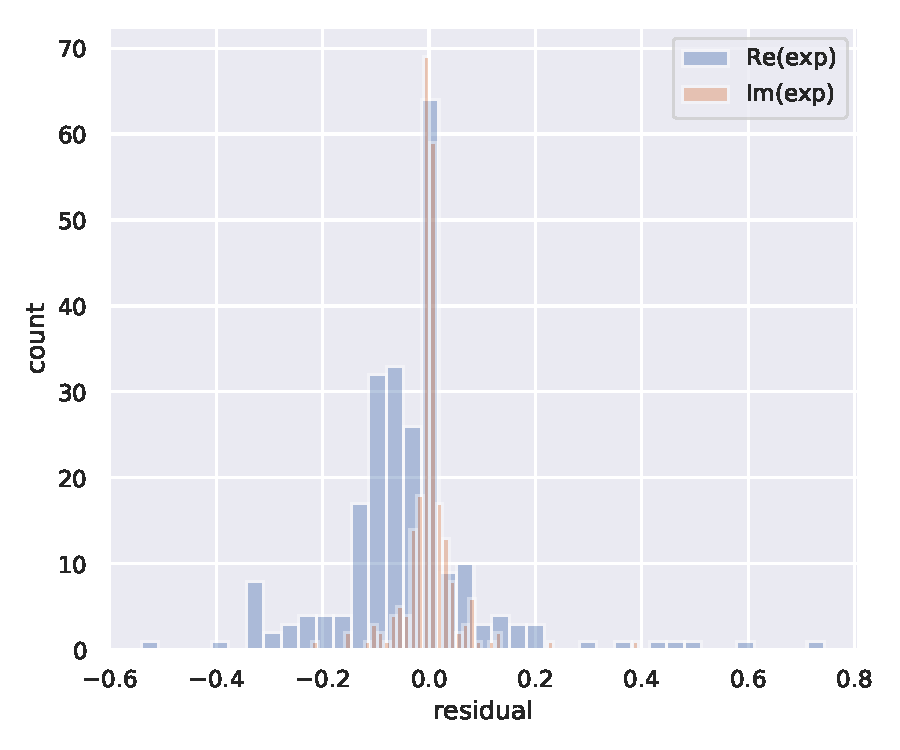
\includegraphics[width=\linewidth]{img/test_res_dist}
    \caption{Univariate distribution.}
  \end{subfigure}
  \begin{subfigure}{0.45\textwidth}
    \centering
    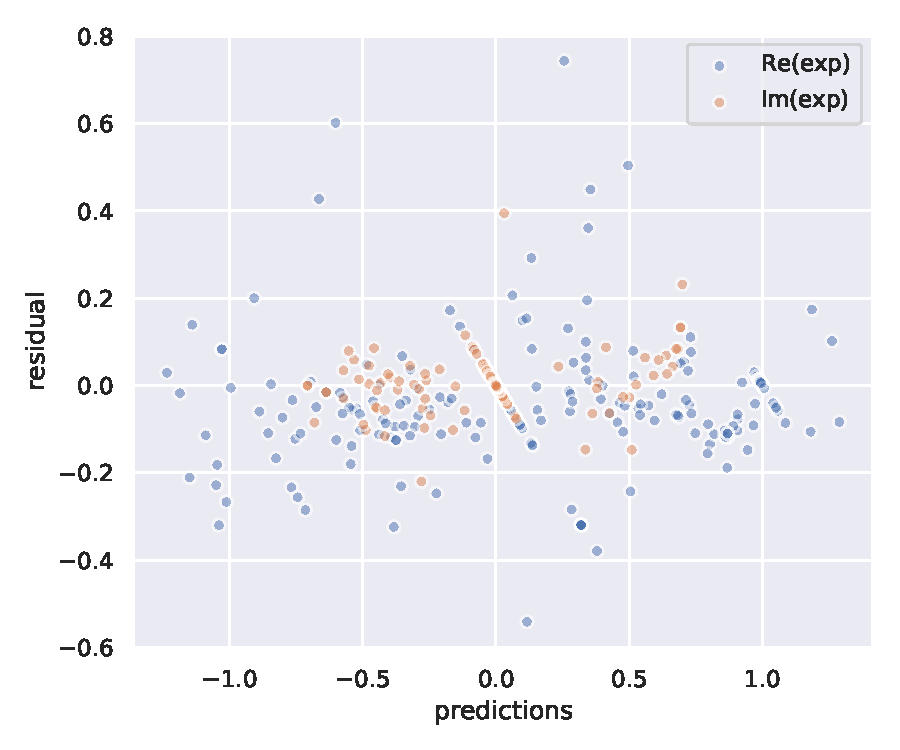
\includegraphics[width=\linewidth]{img/test_res_plot}
    \caption{Residual plot.}
  \end{subfigure}
  \caption{Residuals of the \emph{ANN} model.}
  \label{fig:agg:ann_res}
\end{figure}
